\documentclass{standalone}

\usepackage{newtxtext}
\usepackage{newtxmath}
\usepackage{tikz,pgfplots}
\usetikzlibrary{calc}
\pgfplotsset{compat=1.16}

\begin{document}

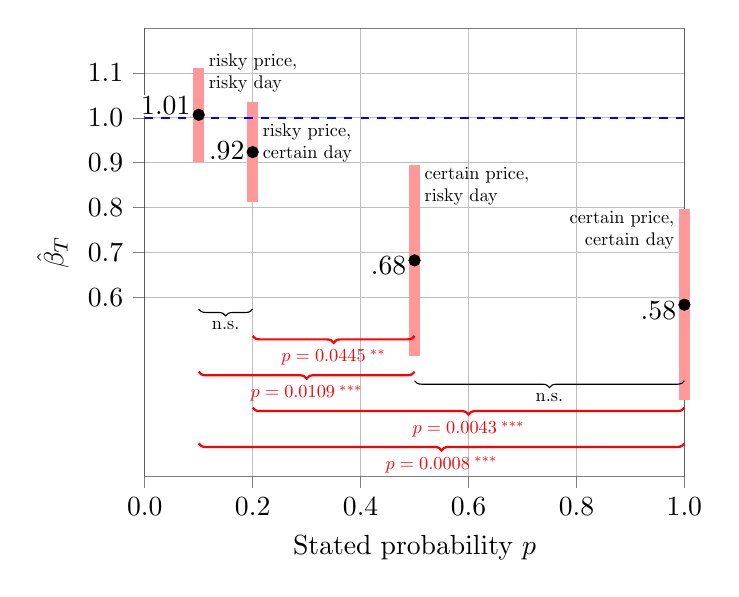
\begin{tikzpicture}[domain=0:1, scale=1]
\begin{axis}[ymin=0.20, ymax=1.2, xmin=0, xmax=1,
  ytick={0.6,0.7,...,1.1}, ytick align=outside, ytick pos=left,
  xtick={0,0.2,...,1}, xtick align=outside, xtick pos=left,
  xlabel=Stated probability $p$,
  ylabel={$\hat\beta_T$},
  axis line style={draw opacity=0.5},
  x tick label style={
                /pgf/number format/fixed,
                /pgf/number format/fixed zerofill,
                /pgf/number format/precision=1},
  y tick label style={
                /pgf/number format/fixed,
                /pgf/number format/fixed zerofill,
                /pgf/number format/precision=1},
  grid=major, clip=false]
\addplot+[
  only marks,
  mark options={black, scale=1},
  visualization depends on=\thisrow{alignment} \as \alignment,
  point meta=explicit symbolic,
  nodes near coords,
  every node near coord/.style={anchor=\alignment,fill=white, inner sep=0.5,outer sep=2.5},
  error bars/.cd, 
    y fixed,
    y dir=both, 
    y explicit,
    error bar style={width=4pt, line width=4pt, white!60!red}
] table [x=x, y=y, y error=error, col sep=comma, row sep=crcr, meta index=3] {
      x,      y,  error, label, alignment\\
    0.1, 1.006907,  0.10403504, 1.01, -16\\
    0.2, 0.9237335, 0.11062103,  .92,  -4\\
    0.5, 0.6821767, 0.2119546,   .68,  12\\
    1.0, 0.5832931, 0.21119,     .58,  12\\
};
\addplot+[no marks,blue,thick,dashed] {1};
\node[right, align=left, scale=0.66, xshift=2pt, yshift=18pt] at ($(axis cs:0.1,1.0276)$) {risky price,\\risky day};
\node[right, align=left, scale=0.66, xshift=2pt, yshift=-4pt] at ($(axis cs:0.2,0.9600)$) {risky price,\\certain day};
\node[right, align=left, scale=0.66, xshift=2pt, yshift=2pt] at ($(axis cs:0.5,0.8393)$) {certain price,\\risky day};
\node[above left, align=right, scale=0.66, xshift=-2pt, yshift=-14pt] at ($(axis cs:1.0,0.7499)$) {certain price,\\certain day};
\draw [decorate,decoration={brace,mirror,raise=4ex},scale=0.2,black]
  (0.5,2.6) -- (1.0,2.6) node[midway,scale=0.66,yshift=-8.2ex]{n.s.};
\draw [decorate,decoration={brace,mirror,raise=4ex},scale=0.2,red,thick]
  (1.0,2.3) -- (2.5,2.3) node[midway,scale=0.66,yshift=-8.8ex]{$p=0.0445^{\;**}$};
\draw [decorate,decoration={brace,mirror,raise=4ex},scale=0.2,red,thick]
  (0.5,1.9) -- (2.5,1.9) node[midway,scale=0.66,yshift=-8.8ex]{$p=0.0109^{\;***}$};
\draw [decorate,decoration={brace,mirror,raise=4ex},scale=0.2,black]
  (2.5,1.8) -- (5.0,1.8) node[midway,scale=0.66,yshift=-8.2ex]{n.s.};
\draw [decorate,decoration={brace,mirror,raise=4ex},scale=0.2,red,thick]
  (1.0,1.5) -- (5.0,1.5) node[midway,scale=0.66,yshift=-8.8ex]{$p=0.0043^{\;***}$};
\draw [decorate,decoration={brace,mirror,raise=4ex},scale=0.2,red,thick]
  (0.5,1.1) -- (5.0,1.1) node[midway,scale=0.66,yshift=-8.8ex]{$p=0.0008^{\;***}$};
\end{axis}
\end{tikzpicture}

\end{document}